% !TEX root = ../thesis.tex
%
\chapter{Experimental Setup}%
\label{sec:experiments}

In order to compare the performance of Software Transactional Memory against Ohua, we employ a set of benchmarks originally proposed by Minh et al.~\cite{minh2008stamp}.
In this chapter, we will categorize the benchmarks introduced by the authors and present a representative selection of applications which we will use to compare Ohua's performance against STM.\todo{Überall noch erwartete Performance bei benches ranschreiben?}
Additionally, we will discuss the values measured during execution of the benchmarks and their relevance for the evaluation.

\section{Benchmark Choice}
\label{sec:experiments:choice}

After presenting our transformations for Ohua in chapter~\ref{sec:transformations}, we now wanted to compare its performance against STM in order to evaluate if Ohua could indeed be used as a suitable replacement for developing parallel irregular applications.
To provide a comprehensive comparison, we chose to use the \emph{Stanford Transactional Applications for Multi-Processing} suite~\cite{minh2008stamp}.
Introduced by Minh et al., it was designed as a set of benchmarks for testing software transactional memory frameworks.
The authors included 8 applications from different application areas in their suite, which are supposed to resemble the diverse landscape of parallelism in applications developers might face.
In particular, the STAMP suite contains examples from different application domains and varying use cases for transactional memory such as high-contention and low-contention scenarios.

\begin{table}
    \centering
    \begin{tabular}{|l|l|l|}
        \hline
        \textbf{Application} & \textbf{Instructions per tx} \emph{(mean)} & \textbf{Time spent in transactions}\\\hline\hline
        labyrinth & 219,571 & 100\%\\\hline
        bayes & 60,584 & 83\%\\\hline
        yada & 9,795 & 100\%\\\hline
        vacation & 3,223 & 86\%\\\hline
        genome & 1,717 & 97\%\\\hline
        intruder & 330 & 33\%\\\hline
        kmeans & 117 & 7\%\\\hline
        ssca2 & 50 & 17\%\\\hline
    \end{tabular}
    \caption{A basic characterization of STAMP applications, comparing the mean number of instructions per transaction and the overall percentage of time the application spends in transactions. These numbers stem from a C implementation and have been adapted from Minh et al.~\cite{minh2008stamp}}
    \label{tab:experiments:overview}
\end{table}

The tables~\ref{tab:experiments:overview} and~\ref{tab:experiments:categorization} give a basic characterization of the benchmarks in terms of their usage of transactions.
As can be seen in table~\ref{tab:experiments:overview}, the length of individual transactions varies greatly per application, as does the overall time that is spent by the benchmark executing transactions.
Even though the numbers in the table have been adapted from Minh et al.\ and represent values measured for their C-based implementation, they still outline the general characteristics of an STM-based algorithm.
Some applications suffer so badly from the irregular properties outlined in chapter~\ref{sec:background:irregular} that exploiting their parallelism requires them to spend more than 80 \% of their overall execution time in transactions.
This is for example the case in the \emph{labyrinth} benchmark, where fields of a dense 3-dimensional matrix have to be continuously updated, as we explained in chapter~\ref{sec:preliminary:labyrinth}.
Other applications such as \emph{kmeans} or \emph{ssca2} have relatively short transactions, meaning their data parallelism is easier to exploit or they generally do not feature as much opportunities for parallelism as other applications.

\begin{table}
    \centering
    \begin{tabular}{|l|l|l|l|l|}
        \hline
        \textbf{Application} & \textbf{tx length} & \textbf{r/w set} & \textbf{tx time} & \textbf{Contention}\\\hline\hline
        labyrinth & long & large & high & high\\\hline
        bayes & long & large & high & high\\\hline
        yada & long & large & high & medium\\\hline
        vacation & medium & medium & high & low/medium\\\hline
        genome & medium & medium & high & low\\\hline
        intruder & short & medium & medium & high\\\hline
        kmeans & short & small & low & low\\\hline
        ssca2 & short & small & low & low\\\hline
    \end{tabular}
    \caption{A qualitative summary of each STAMP application's runtime transactional characteristics. The length of a transaction is determined by the number of instructions it encompasses. The characteristics are ranked relative to the other applications in the suite. Adapted from Minh et al.~\cite{minh2008stamp}}
    \label{tab:experiments:categorization}
\end{table}

Another relevant and perhaps the most limiting factor for programs relying on optimistic parallelism principles such as STM is contention.
This characteristic is visualized in table~\ref{tab:experiments:categorization} along with other properties.
When facing high contention scenarios, STM implementations are usually unable to achieve the near-linear speedups Minh et al.\ reported for other benchmarks.
Contention is a byproduct of frequent reading and writing accesses to the shared data structure that inevitably lead to frequent conflicts which require a rollback of all affected threads except for the one that committed its changes first.
Hence, the relative amount of reads and writes per transaction is also reported in table~\ref{tab:experiments:categorization}.
Long transactions, large read/write sets, more time spent in transactions and high contention are all factors promoting conflicts.
The results of conflicts are frequent rollbacks and accompanying recomputations, which reduce the overall performance.

Based on the analysis provided by the authors, we selected a representative range of benchmarks for our comparison between Ohua and STM.
We chose applications with varying transaction lengths and frequency of transaction use as well as different levels of contention.
The next sections will briefly outline the details of the chosen benchmarks and explain, how they were implemented.


% THEN elaborate further about the technical details that hold true for all benchmarks
Since the authors only provided a C-based reference implementation for their programs, we had to re-implement them in Rust to rule out language-specific performance changes when comparing to Ohua's Rust implementation.
Upon inspecting the original source code, it turned out that the authors adapted the code in order to improve the performance of STM in some benchmarks.
For instance, they provided their own implementation of a \rust{HashMap}\footnote{A dynamic key-value store allowing fast lookups by hashing the keys and organizing them in different buckets.} that offered the use of transactions on a per-bucket basis, effectively exposing fine-granular parallelization opportunities that normal HashMaps cannot provide.
In Rust, no corresponding STM-specific data structures existed prior to this work.
We debated, whether or not we should use these optimizations in our own implementation but ultimately decided in favor of doing so.
First, one could argue that these optimizations would be made by developers anyway after deciding to use the STM framework in an attempt to tailor the program code towards the library used.
Secondly, we wanted to remain as close as possible to the original implementations from Minh et al.\ in the hopes of achieving similar results for STM as they did.
Therefore, we contributed a small library~\cite{wittwer2020stmdata} which provides data structures like HashMaps and HashSets augmented for the use with transactions.
Both the library and the benchmarks were implemented from scratch based on the descriptions provided by the authors, literature they cited and the code they supplied.
We did so in an idiomatic way, applying both concepts to the problems using the tools the frameworks and the STM data structure library provide natively.\todo{Link the rust-stm repository here -> which changes have i made?}


%TODO:
%- explain why i chose bench xy
%- explain benches
%  - detail for labyrinth (etc) why they are so hard to parallelise

\subsection{Labyrinth Path Mapping}
\label{sec:experiments:labyrinth}

The labyrinth benchmark we presented in chapter~\ref{sec:preliminaries:labyrinth} based on the work of Swalens et al.~\cite{swalens2016transactional} was originally proposed by Minh et al. as possible benchmark for Software Transactional Memory.
Since we have already analyzed and implemented this application, it was apparent for us to adduce it for our concluding comparison.
Additionally, is is one of very few\todo{check again if that's the case!} benchmarks in the suite exhibiting amorphous data parallelism, a trait the authors did not consider when compiling their benchmark list but which they happened to include by coincidence, as it is frequently encountered in real-life applications using shared state, the main use case for transactional memory applications.
Another interesting property of the benchmark was its frequent use of transactions (the whole algorithm is executed within transactions) and the high contention on the shared data structure, which puts the synchronization primitives under heavy stress.

\todo{Braucht es noch Anmkerungen, warum das hier interessant ist?}


%The \emph{labyrinth} benchmark implements a variation of Lee's algorithm \cite{lee1961algorithm} which was conceived to solve path-connection problems that often arise e.g., when searching for an optimal route or when constructing wiring diagrams in electrical engineering.
%Watson et al.~\cite{watson2007study} were the first to implement the algorithm using transactional memory techniques to measure the performance on such systems.
%Based of their algorithm description, we implemented the benchmark, as it has been described in chapter~\ref{sec:preliminary}\todo{verify correctness of this link}.
%\todo{complete this: Ohua-Impl -> was ist parallel?, original perf \& expected perf}

\subsection{Intruder Detection}
\label{sec:experiments:intruder}

The intruder application implements a signature-based Network Intrusion Detection System (NIDS) and is used in networking to detect attacks or malicious activities in an active network as well as policy violations.
It is based on design proposal number five of Haagdorens et al.'s work on \enquote{Improving the Performance of Signature-Based Network Intrusion Detection Sensorz by Multi-Threading}~\cite{haagdorens2004improving}.

The basic function of this application is to scan incoming network packets and match them against known intrusion signatures.
This happens in three distinct stages, as outlined in Fig.~\ref{fig:experiments:intruder:workflow}.
Incoming network traffic is captures and queued for inspection.
Due to the architecture of modern network protocols, individual data flows have to be split into several packets that are transmitted individually and may reach the recipient out of order.
Attackers have used this in the past by splitting malicious flows and sending them out of order to avoid detection.
To counter this, the second step in the algorithm is to deploy stateful detection avoidance countermeasures, which involve preprocessing the received packets and reassembling the original flows.
These flows can then finally be matched against known attack patterns, filtering any malicious packets from the stream of incoming data.

\begin{figure}
    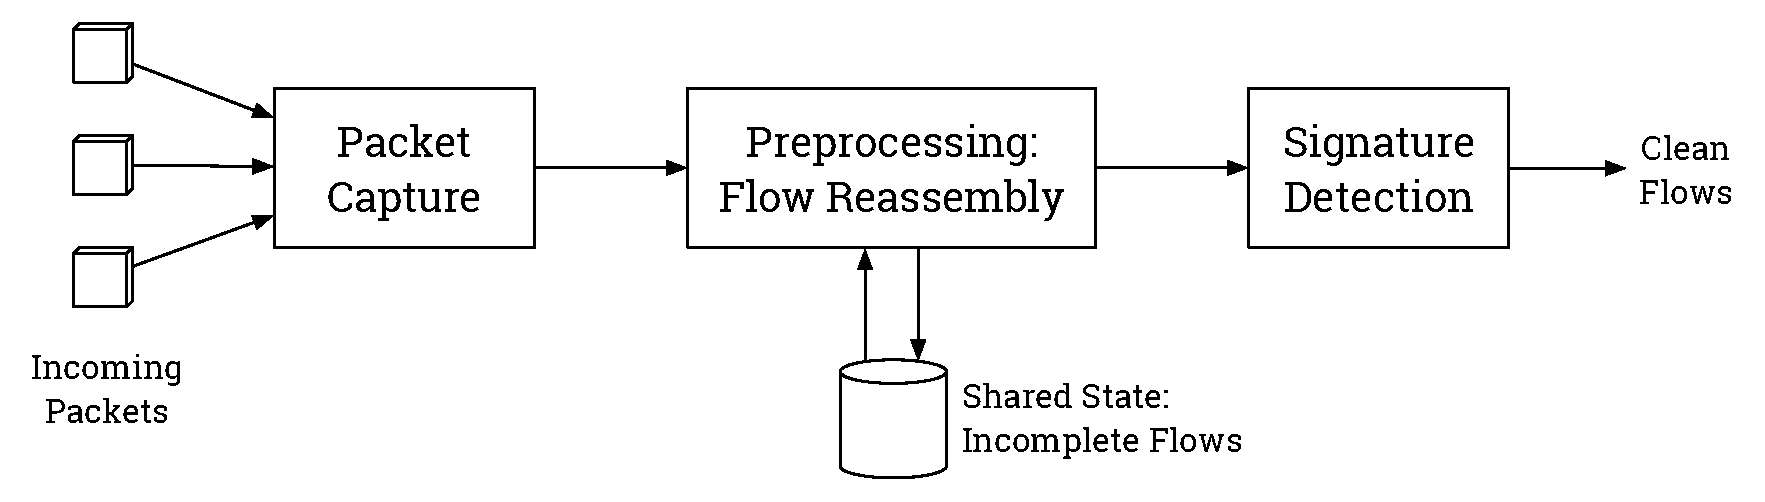
\includegraphics[width=\textwidth,keepaspectratio]{gfx/experiments-intruder}
    \caption{Workflow of the Intruder Benchmark. Processing of incoming data is conducted in three stages.}%
    \label{fig:experiments:intruder:workflow}
\end{figure}

While our STM implementation performs the steps two and three in parallel, in Ohua only the thirs step is parallelized by the compiler since the second step consists only of a loop that appends all inputs to a state value.
Since the loop body does not contain any other state-free functions, no transformations from chapter~\ref{sec:transformations} may be applied.
Step three however consists of a state-free loop where all inputs are checked for malicious data flows, something that can easily be optimized by applying transformation one as presented in chapter~\ref{sec:transformations:tf1}.
This shows that Ohua may only extract parallelism from irregular applications that fit certain criteria, i.e., contain loops that do not only contain state-modifying operations, as its main approach is to exploit data parallelism by the use of certain transformations to uncover it.

This benchmark was chosen because it is mostly similar in its properties to the labyrinth application as it also features short transactions and high contention on the shared data, but does only spend about 33 \% of the overall execution time in transactions.
We mainly wanted to see, how this slight difference in properties is reflected in the performance results.


\subsection{K-means Clustering}
\label{sec:experiments:kmeans}

Proposed as benchmark by Narayanan et al.~\cite{narayanan2006minebench} the k-means clustering algorithm partitions a set of $n$ observations into $k$ clusters.
It was originally put forth by MacQueen et al. in 1967~\cite{macqueen1967some} and still is a very popular algorithm for cluster analysis in data mining which is often used to classify data.

The inner workings of the algorithm are rather simple: It takes a set of $n$ observations and a desired number of clusters to sort the observations into.
Then the $k$ cluster centroids are initialized.
Many ways exist to realize this but we chose, akin to our C reference implementation, to select each coordinate for each cluster centroid randomly from the coordinates preset by the input data set.
Following this initialization, each observation is assigned to its nearest cluster based on the squared multi-dimensional spatial euclidian distance between both points.
Afterwards, new centroids are computed by calculating the means of all observations now assigned to a certain cluster.
These last two steps now get repeated iteratively until the algorithm either reaches an upper bound of iterations or converges, i.e., less than a certain percentage of observations change per iteration.

In STM each iteration is executed completely in parallel, splitting the input dataset equally among the executing threads and guarding access to the centroids and the delta value which is used for deciding on convergence using transactions.
Ohua also does each iteration in parallel using transformations one and three\todo{Numbering ok like this? Has afaik never been officially established} to exploit data parallelism although the loop has been written in the algorithm in a way to make sure no shared state exists within.

k-means is very much like the intruder benchmark in the regard that its parallelism opportunities are limited to a single state-free loop but unlike the aforementioned benchmark k-means features low contention on shared data structures while presenting a similar transaction utilization, making this an interesting benchmark to look at.

\subsection{Genome Sequencing}
\label{sec:experiments:genome}
This benchmark implements a \emph{\enquote{whole-genome shotgun sequencing}} algorithm as outlined by Pop et al.~\cite{pop2002genome} in their work.
Its goal is to sequence a (fictional) genome, i.e.\ to reassemble a nucleotide sequence from a set of snippets which is something frequently done in genetics.

\begin{figure}[b]
    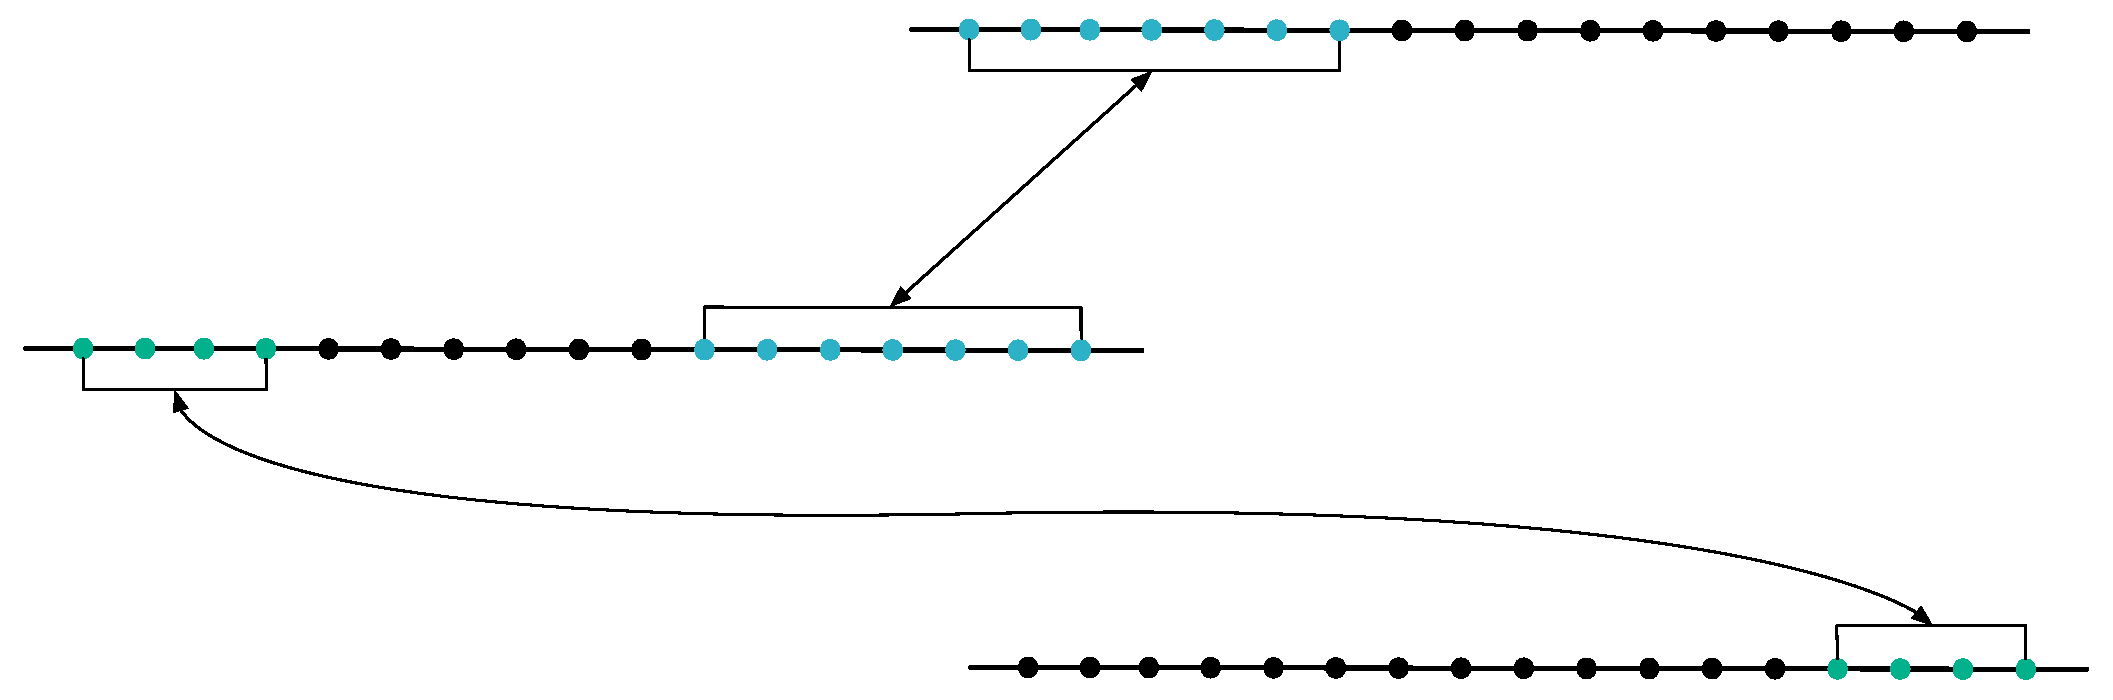
\includegraphics[width=\textwidth,keepaspectratio]{gfx/experiments-genome}
    \caption{Visualization of the overlap matching found in the genome benchmark. The blue match is stronger as it has seven matching elements and has hence been found first.}
    \label{fig:experiments:genome-example}
\end{figure}

The first step in the algorithm is to deduplicate the DNA segments that have been provided as inputs, since there are usually many duplications.
The second phase is then concerned with finding neighboring segments in the remaining pool of DNA parts by utilizing overlap matching.
By reducing the overlap size each iteration, the best possible fit is chosen for each neighbor search.
Figure~\ref{fig:experiments:genome-example} provides visualization of how this matching works.
Starting from a match length of $n-1$, the algorithm attempts to find a matching predecessor-successor pair for all loose ends.
With each iteration, the match length is reduced, until it ends with an overlap of one.
In our example, the blue overlap match is found first due to seven matching nucleotides.
Three iterations later, the green match is established, fully connecting the centered genome segment.
After this phase has finished, all but two segments have a predecessor and successor assigned.
Starting from the one element in the set with no predecessor, the chain of nucleotides can be rebuilt by simply following the links.

In STM, the deduplication phase as well as the matching phase are implemented in parallel using a transaction-aware hash set implementation for the first and a doubly-linked list for the latter.
Although we cannot provide an implementation for a hash set that can be shared using Ohua, we opted to assist the compiler in uncovering parallelism in the deduplication step by manually partitioning the worklist beforehand, so that the compiler may break the resulting state-free loop using the first transformation:
\begin{minted}{Rust}
fn dedup(segments: Segments, threadcount: usize) -> Vec<SequencerItem> {
    let parts = partition(segments, threadcount);
    for p in parts {
        deduplicate(p)
    }
}
\end{minted}
The second step is also a simple state-free loop, which can be easily parallelized by just applying transformation four.
This application example shows, that even when using Ohua, code sometimes has to be written in a certain way to expose the parallelism opportunities of a computation to the compiler.
Nevertheless, the resulting Ohua algorithms can still be executed as a sequential program while the resulting STM code which is even more optimized by the use of special data structures, is unable to do so.

Overall we chose this application to complete our benchmark selection as it provides similar properties as the kmeans benchmark in terms of transaction length and contention but spends nearly all its execution time in transactions, a stark change compared to the 7 \% of transaction time in kmeans.



% - Part 1: Benchmark Choice
%   - which benchmarks did I choose for my thesis, and why? outline the parameters and reasons for the decision
%   - discuss parameters we used to run the benchmarks
%   - Give short overview over the used benchmarks

\section{Measurements}
\label{sec:experiments:measurements}

In our experiments, we tried to achieve reproducible and plausible results so that we can make an educated comparison between both STM and Ohua.
This section will briefly explain our benchmarking setup to enable others to reproduce our results.

\subsection{Input Data}
\label{sec:experiments:measurements:inputs}

For each STAMP application, Minh et al.~\cite{minh2008stamp} also provided three sets of parameters to model small, medium and large workloads.
We adopted these parameters with only minor modifications, as intended by the authors.
A change was made to the parameters of the \texttt{genome} benchmark as the input data that was randomly created using the original input parameters proved faulty in our re-implementation.
Also, a unnecessary parameter was removed from the \texttt{kmeans} benchmark.

\begin{table}
    \centering
    \tiny
    \begin{tabular}{|l l l|}
        \hline
        \textbf{Application} & \textbf{Arguments} & \textbf{Description}\\\hline\hline
        genome & -g 256 -s 16 -n 16384 & \multirow{3}{*}{\begin{minipage}{.4\textwidth}$n$ gene segments of length $s$ are first sampled from a gene consisting of $g$ nucleotides and then reassembled again.\end{minipage}}\\
        genome+ & -g 510 -s 32 -n 32768 & \\
        genome++ & -g 16384 -s 64 -n 16777216 & \\\hline

        intruder & -a 10 -l 4 -n 2048 -s 1 & \multirow{3}{*}{\begin{minipage}{.4\textwidth}From seed $s$, $n$ traffic flows are generated, $a\%$ of which contain attacks. Each flow consists of up to $l$ packets, which are assembled and inspected by the program.\end{minipage}}\\
        intruder+ & -a 10 -l 16 -n 4096 -s 1 & \\
        intruder++ & -a 10 -l 128 -n 262144 -s 1 & \\\hline

        kmeans-high & -n 15 -t 0.05 -i random-n2048-d16-c16.txt & \multirow{6}{*}{\begin{minipage}{.4\textwidth}The input file $i$ containing $n$ points in $d$ dimensions generated about $c$ centers is loaded and then clustered into $n$ clusters. A convergence threshold of $t$ is used.\end{minipage}}\\
        kmeans-high+ & -n 15 -t 0.05 -i random-n16384-d24-c16.txt & \\
        kmeans-high++ & -n 15 -t 0.00001 -i random-n65536-d32-c16.txt & \\
        kmeans-low & -n 40 -t 0.05 -i random-n2048-d16-c16.txt & \\
        kmeans-low+ & -n 40 -t 0.05 -i random-n16384-d24-c16.txt & \\
        kmeans-low++ & -n 40 -t 0.00001 -i random-n65536-d32-c16.txt & \\\hline

        labyrinth & -i random-x32-y32-z3-n96.txt & \multirow{3}{*}{\begin{minipage}{.4\textwidth}The input file $i$ describes a maze of dimensions $x \times y \times z$ and $n$ paths to map.\end{minipage}}\\
        labyrinth+ & -i random-x48-y48-z3-n64.txt & \\
        labyrinth++ & -i random-x512-y512-z7-n512.txt & \\\hline
    \end{tabular}

    \caption{Input data sets for the benchmarks presented in this thesis. Adapted from Minh et al.~\cite{minh2008stamp} and adjusted to mitigate flaws in the original algorithms.}
    \label{tab:experiments:inputs}
\end{table}

Table~\ref{tab:experiments:inputs} gives a full overview over all parameters we used.\todo{Verify correctness of values and parameters(!)}
Input sets marked with a + indicate a larger input and an appended ++ marks the largest of the three input sets for a benchmark.
The \texttt{kmeans} benchmark inputs are additionally labeled as \emph{high} and \emph{low}, which refers to the relative amount of contention produced by the inputs.

\subsection{Measured Values}
\label{sec:experiments:measurements:values}

For the purpose of our comparison between Ohua and STM, two values are of importance and have hence been measured.
As we are calculating the speedups of both implementation in reference to a sequential implementation, the execution time in milliseconds, i.e., the time it takes the algorithm to complete, is relevant.
Moreover, we were interested in the power consumption of both algorithms.
But since measuring the power consumption of the algorithms would have been to complicated and time-consuming, we opted for measuring the total CPU time used by the programs, as the amount of power used while processing is resulting from the utilization of a PCs individual components.
Since all these programs are performing purely in-memory computations, we figured that measuring the CPU time would be a sufficient approximation to draw some general conclusions regarding the power usage.

For both measured values, the setup phase (parsing input arguments and reading input files) and teardown phase (writing the results to a file) where not included in the measurements.
This was done in order to reduce potential noise from Operating System calls resulting from the I/O operations performed in these stages.\todo{Evtl. über Genauigkeit bei Messungen reden? (Messung in ms, messfehler, ...)}
Research has shown in the past that this noise, as well as different contention scenarios can severely impact the measured time values, leading to variations in the measured time values.
To take this into account and produce more realistic results, each measurement has been done 30 times, to that statistical outliers do not carry as much weight.
From the resulting measured values the geometric mean was calculated per data point to compile all measurements into a single data point.

\subsection{Running Configuration}
\label{sec:experiments:measurements:hardware}

All benchmarks conducted for this work were run on an Ubuntu 18.04 server with 128GB RAM and two Intel Xeon E5-2630 v2 processors which have a base frequency of 2.60 GHz and offer combined 12 cores with 24 threads.
At all times, the program under inspection was running exclusively on the machine, meaning that aside from background operating system jobs, no other tasks ran on the system simultaneously.\todo{keep out to have this as source for errors?}

\subsection{Reference Measurements}
\label{sec:experiments:measurements:reference}

\todo{Make section?}
Minh et al.\ proposed their STAMP suite in 2008.
Since then, hardware (e.g., clock speeds of CPUs) as well as compile-time optimizations have evolved significantly, rendering the results provided in their paper outdated.
Hence, we decided to run the benchmarks relevant to our investigation again, on the same hardware and under the same conditions as our Rust benchmarks to have a reference we can compare our STM implementations to.
Although the authors themselves only measured results for the smaller two of their three suggested input sets, we tested all three to have a more comprehensive set of results to compare our STM implementation against.\todo{ok?}

Upon building and executing the benchmarks with the included \texttt{tl2} STM implementation, a number of issues with the STAMP suite became apparent, which we already briefly touched upon in chapter~\ref{sec:introduction}.
The genome benchmark could not be built from the original source code, due to conflicts caused by compile-time memory allocation patching.
We reported this issue~\cite{wittwer2020stampgenome} and employed a workaround to be able to use the benchmark nonetheless.
Additionally, we found that the implementation of the labyrinth benchmark sometimes does not yield a correct solution, causing the program to crash.\todo{report?}
Similar behavior was found for the intruder application, although we did not investigate this further, instead discarding failed runs in both cases, owering the effective number of test results slightly below 30.
These issues cement some of the drawbacks of STAMP and STM in general, which we discussed in the beginning of this thesis.

For comparability and in order to provide a more complete performance graph, we intended to run the selected four benchmarks also for 1-24 threads but the suite only supports thread counts which are a power of two, leaving us with 1, 2, 4, 8 and 16 threads as test parameters.
Due to this limited result range, we will only be able to draw vague general comparisons between STAMPs STM and our own STM implementation as the sparse result coverage for higher thread counts leaves us unable to reliably identify trends in the performance of STAMP.

